% This is samplepaper.tex, a sample chapter demonstrating the
% LLNCS macro package for Springer Computer Science proceedings;
% Version 2.21 of 2022/01/12
%
\documentclass[runningheads]{llncs}
%
\usepackage[T1]{fontenc}

% T1 fonts will be used to generate the final print and online PDFs,
% so please use T1 fonts in your manuscript whenever possible.
% Other font encondings may result in incorrect characters.
%
\usepackage{graphicx}
% Used for displaying a sample figure. If possible, figure files should
% be included in EPS format.
%
% If you use the hyperref package, please uncomment the following two lines
% to display URLs in blue roman font according to Springer's eBook style:
%\usepackage{color}
%\renewcommand\UrlFont{\color{blue}\rmfamily}
%\urlstyle{rm}
%
\begin{document}
%
\title{Automated Research Paper Discovery and Recommendation through Citation and Metadata Analysis}

\author{
    Amna Shahid\inst{1} \and 
    Fatima Qurban\inst{1} \and 
    Mohammad Eman\inst{1}
    \newline
    \authorinfo{
    {i211148@nu.edu.pk}
}
\authorinfo{
    {i211195@nu.edu.pk}
}
\authorinfo{
    {i211140@nu.edu.pk}
}
}

\institute{
    National University of Computer and Emerging Sciences (NUCES), Islamabad, Pakistan
}

\maketitle     


\begin{abstract}
In the era of exponential research output, efficiently discovering and recommending relevant academic papers is a growing challenge. This paper presents a novel system for automated research paper discovery and recommendation through citation and metadata analysis, leveraging Natural Language Processing (NLP) techniques and advanced similarity matching models. The system allows users to input a research paper's title or DOI, after which it fetches the paper’s metadata, including citations and references, using the Semantic Scholar API. To enable comprehensive filtering and similarity-based recommendations, we developed a model using the SentenceTransformer (all-MiniLM-L6-v2) for embedding titles and abstracts. Similarity searches are conducted using FAISS (Facebook AI Similarity Search) indices, enabling rapid identification of related research papers.

Our approach includes basic string-matching techniques for author similarity and model-based comparisons for title and abstract similarity. The system provides visual insights through t-SNE plots and similarity matrices to enhance user understanding of the relationships among the recommended papers. Furthermore, a React-based front-end application allows users to input titles or DOIs, view metadata, and explore recommendations interactively. This research demonstrates the effectiveness of combining NLP-driven embedding models, citation analysis, and interactive visualization for improving the efficiency of research paper discovery and recommendation. The proposed system can significantly aid researchers in navigating extensive literature, identifying relevant work, and fostering more efficient knowledge discovery.
\newline
\end{abstract}
\textit{\textbf{Keywords}: Research Papers, Paper Discovery, Citation Analysis, NLP, FAISS, Semantic Scholar, Recommendation System}
\section{\textbf{Problem Statement}}
Finding and selecting pertinent publications is becoming increasingly difficult for academics as the amount of academic research is increasing at an exponential rate. The amount and complexity of the available literature make traditional search techniques—which rely on keyword matching and human filtering—inadequate. The research process is hampered by this inefficiency, which slows the finding of new information and raises the possibility of missing important studies.There is a need for an automated solution that leverages advanced Natural Language Processing (NLP) techniques, citation analysis, and interactive visualization to streamline research paper discovery and recommendation, ensuring that researchers can quickly and accurately find the most pertinent academic works.
\section{\textbf{Introduction}}
The number of academic papers is increasing as never-before in the current research environment. Every day, thousands of new articles are produced in disciplines including engineering, computer science, and medicine. Although this increase in research output is good for knowledge advancement, it poses a big problem for researchers who must quickly find pertinent work. Because of the large volume and complexity of the accessible papers, traditional approaches for finding research papers such as keyword-based search engines and manual citation exploration are becoming less and less effective. This inefficiency raises the possibility of overlooking crucial research, prevents  collaboration, and delays scientific advancement.

Furthermore, a large number of current discovery systems fail to adequately utilize the rich metadata found in research articles, including authorship, abstracts, references, and citations. Citation relationships and metadata analysis offer important  context that can improve the precision of research paper suggestions.  But a vast majority of existing technologies ignore deeper linguistic and contextual linkages that can show more complex connections between publications in favor of simple keyword matching. Our system generates title and abstract embeddings by utilizing Natural Language Processing (NLP) techniques, notably the SentenceTransformer model. The system can swiftly find and suggest publications based on citation and metadata analysis by combining FAISS (Facebook AI Similarity Search) for effective similarity searches.

Our approach attempts to assist researchers in navigating the constantly growing corpus of research papers by resolving the drawbacks of conventional search methods and integrating cutting-edge strategies. By promoting creativity and cooperation among the research community, this study aids in the creation of more potent instruments for knowledge discovery.

\section{\textbf{Related Work}}
The development of advanced recommendation systems that can effectively guide scholars and find pertinent research papers has become necessary due to the exponential rise of the scientific literature. Several strategies have been investigated in the past to tackle this problem, and each has added something special to the field of academic paper recommendation.
The main goal of current recommendation systems \cite{r2} has been to enhance paper discovery and recommendation by utilizing several strategies.

\textbf{Content-Based Filtering:} Numerous systems use content-based methodologies that examine research articles' textual features. To determine the similarity of research articles and capture the semantic meaning of documents, these approaches usually employ strategies like Term Frequency-Inverse Document Frequency (TF-IDF).
\newline
\textbf{Similarity Metrics}: Researchers have investigated various similarity computation methods, with cosine similarity emerging as a popular approach for measuring the semantic relatedness of documents. This metric allows for quantifying the similarity between research papers based on their feature vectors.

To address the challenge of high-dimensional data, researchers have employed dimensionality reduction methods such as t-Distributed Stochastic Neighbor Embedding (t-SNE) has been used for displaying high-dimensional data in a two-dimensional space and Principal Component Analysis (PCA) for lowering feature dimensions while maintaining the majority of the original variance.
These methods aid in the management of intricate, multi-dimensional research paper representations.

In the past, recommender system research has generally depended on methods like content-based filtering, collaborative filtering, or hybrid approaches. By offering a more semantically rich approach to identifying research interests and suggesting pertinent documents, Chandrasekaran et al\cite{r1}.'s study adds to this body of knowledge.

\begin{itemize}
    \item Citation network analysis
    \item Topic modeling
    \item Machine learning-based recommendation algorithms
    \item Semantic similarity measures
\end{itemize}
The approach proposed by Chandrasekaran et al \cite{r1}. distinguishes itself by its focus on conceptual representation and tree-edit distance, offering a more sophisticated method for understanding research similarities beyond traditional keyword or citation-based approaches.

\section{\textbf{Proposed Method}}

The objective of our approach is to identify the details of the research paper, about which the details (DOI or title) has been given as input, fetch all the papers that has cited that specific paper, prompt the user to search the related papers based on three types of metrics: Title, Authors and Abstract similarities. We are then recommending the most relevant papers which are present in our metadata to the user, using Sentence Transformer Models like all-MiniLM-L6-v2 and FAISS.
\begin{figure}
    \centering
    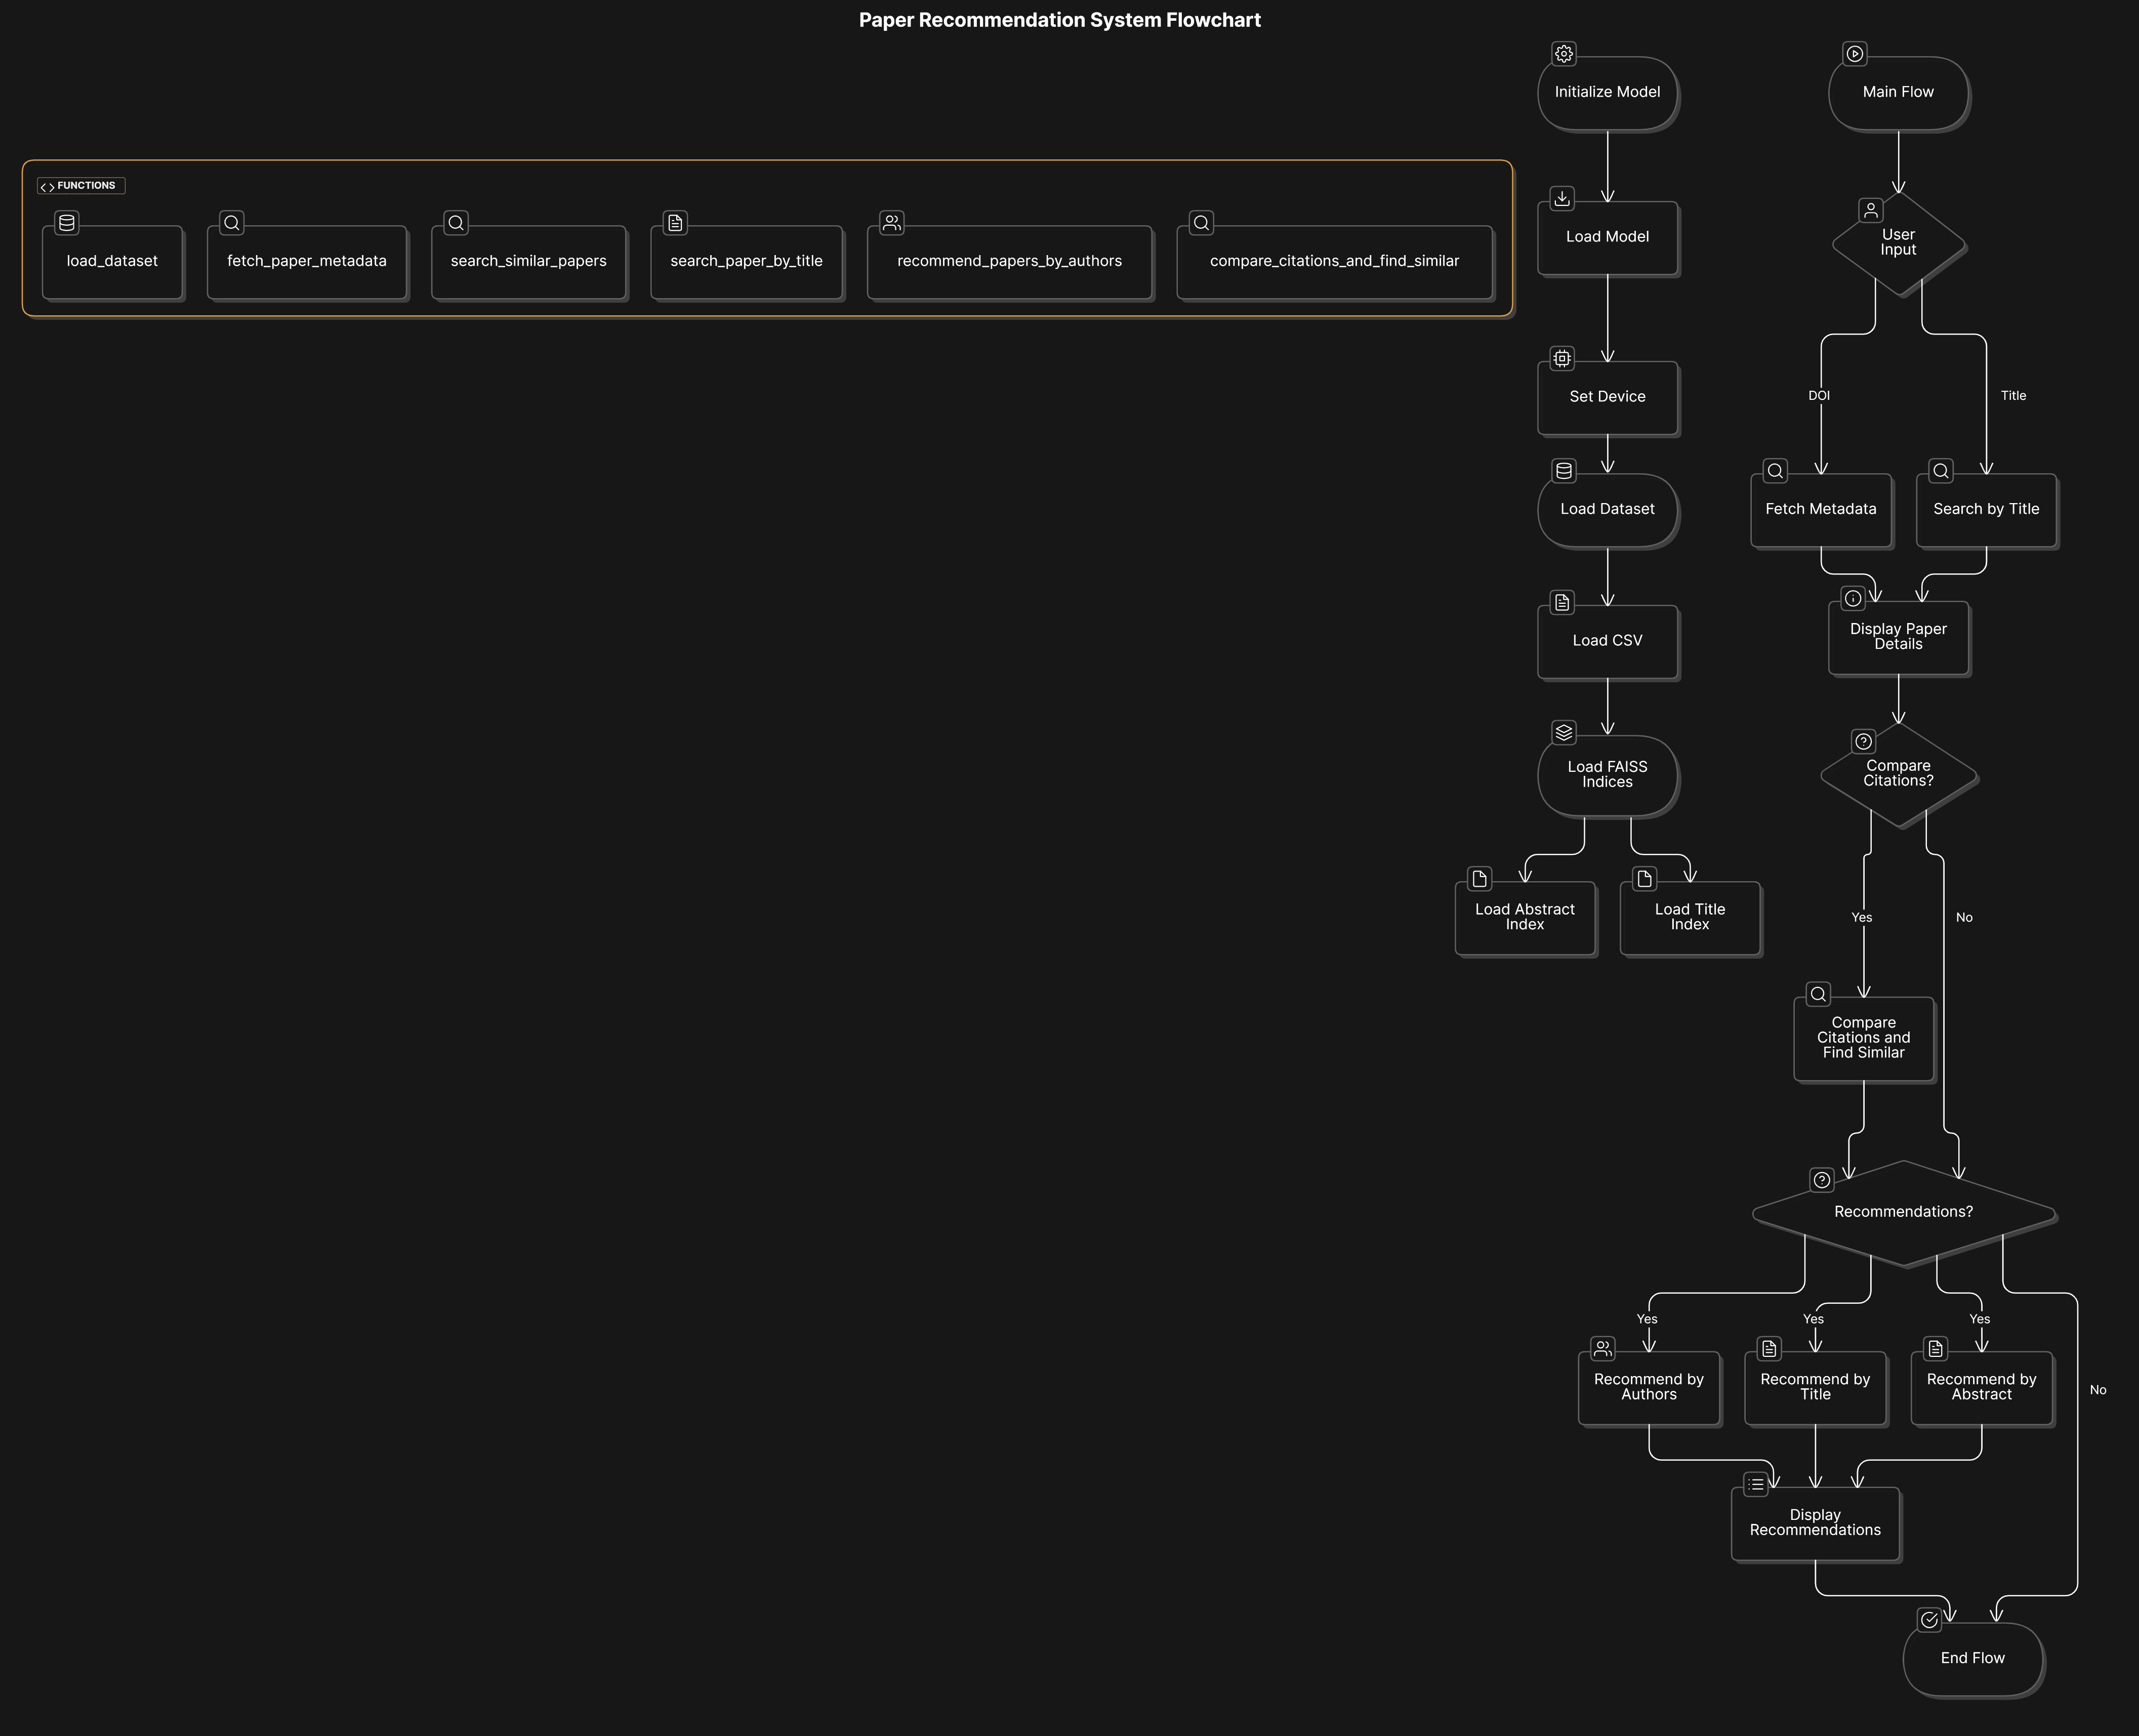
\includegraphics[width=1\linewidth]{System flow.png}
    \caption{System Flow Chart}
    \label{fig1}
\end{figure}

\subsection{\textbf{Data Collection}}
For developing our Research Paper Recommendation System, we used the DBLP dataset (Version 10) from Kaggle as our primary data source. This dataset provides an ample and wide collection of research papers across different domains.
The DBLP dataset offers a comprehensive compilation of research papers with extensive metadata, enabling robust analysis and recommendation strategies. 
Dataset Characteristics:
The dataset comprises multiple attributes for each research paper:
\begin{itemize}
\item \textbf{Unique Identifier:} A distinct \texttt{id} for precise paper referencing
\item \textbf{Publication Metadata:}
\begin{itemize}
\item Title:Complete research paper title
\item Authors: Comprehensive list of paper contributors
\item Venue: Publication platform or journal
\item Publication Year: Temporal information of research
\end{itemize}
\item \textbf{Citation Metrics:}
\begin{itemize}
\item \textit{Citation Count:} Number of times the paper has been referenced
\item \textit{References:} List of cited paper identifiers
\end{itemize}
\item \textbf{Textual Content:} Abstract providing a concise overview of the research
\end{itemize}

\subsection{\textbf{Model training and classification}}
Our research paper recommender system integrates advanced Natural Language Processing (NLP) and machine learning techniques to generate semantically meaningful and accurate research paper recommendations.
\subsubsection*{NLP Techniques}
We transformed research papers using state-of-the-art embedding techniques:
\begin{itemize}
\item \textbf{Sentence Embeddings:} Converted research paper titles, abstracts, and queries into dense, semantically rich vector representations using \texttt{sentence-transformers}, enabling deep semantic understanding beyond traditional keyword matching.
\end{itemize}
\subsubsection*{Recommendation Strategies}
Our recommendation framework employed multiple complementary approaches to ensure comprehensive and precise recommendations:
\begin{itemize}
\item \textbf{Similarity-Based Recommendations:}
\begin{itemize}
\item Developed sophisticated text similarity techniques to measure semantic closeness between research papers
\item Implemented robust author matching algorithms to leverage collaborative filtering principles
\item Utilized FAISS and advanced regular expressions to enable precise and efficient similarity matching
\end{itemize}
\end{itemize}
\subsubsection*{Visualization Techniques}
We enhanced recommendation interpretability through advanced data visualization:
\begin{itemize}
\item \textbf{Similarity Visualization:}
\begin{itemize}
\item Generated informative heatmaps using Seaborn to represent similarity distributions
\item Created interactive scatter plots with Plotly to visualize paper relationships in reduced dimensional space
\item Developed comprehensive visualizations to illustrate similarity scores and clustering patterns
\end{itemize}
\end{itemize}
\subsubsection*{Implementation Framework}
The recommender system leveraged a robust technological ecosystem:
\begin{itemize}
\item \textbf{Machine Learning:} Utilized scikit-learn for statistical modeling and UMAP for advanced dimensionality reduction
\item \textbf{Visualization:} Integrated Seaborn, Plotly, and Matplotlib for comprehensive data representation
\item \textbf{NLP:} Employed sentence-transformers for semantic embedding and FAISS for efficient similarity search
\item \textbf{Data Manipulation:} Processed and transformed data using Pandas and NumPy
\end{itemize}
\subsubsection*{Recommendation Workflow}
The recommendation process follows a systematic and user-centric approach:
\begin{enumerate}
\item User initiates recommendation by providing a research paper identifier
\item Retrieve and parse comprehensive paper metadata from the dataset
\item Optionally perform advanced citation and semantic similarity comparisons
\item Generate personalized recommendations through multiple strategies:
\begin{itemize}
\item Author-based similarity matching
\item Semantic similarity based on paper titles
\item Semantic similarity derived from paper abstracts
\end{itemize}
\item Visualize recommendations using advanced dimensionality reduction techniques
\end{enumerate}
\subsubsection*{Key Algorithmic Components}
Critical algorithmic innovations driving our recommendation system:
\begin{itemize}
\item Semantic embedding generation to capture nuanced research paper characteristics
\item Euclidean distance-based similarity calculation for precise paper matching
\item Non-linear dimensionality reduction using t-SNE and UMAP for complex data visualization
\item Efficient similarity search enabled by Faiss indexing techniques
\end{itemize}


\begin{figure}
    \centering
    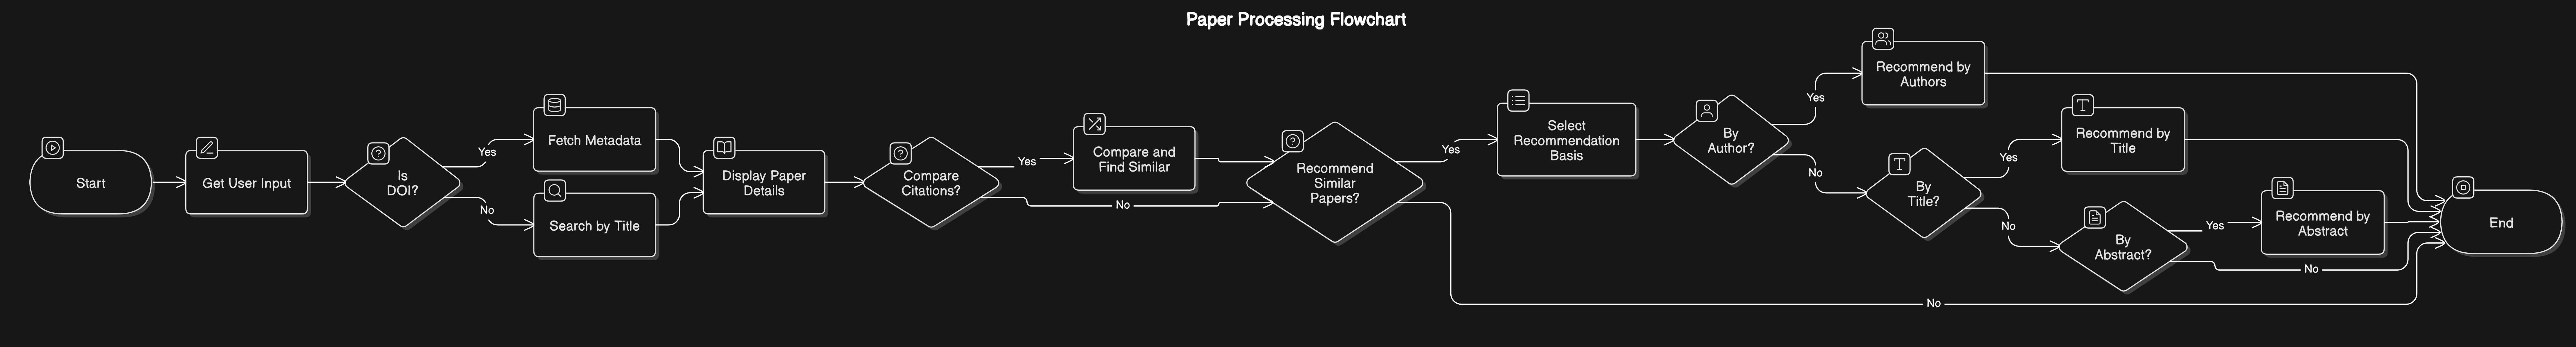
\includegraphics[width=1\linewidth]{paper processing flow.png}
    \caption{Paper Processing Flow}
    \label{fig1}
\end{figure}

\section{\textbf{Evaluation and Experimentation}}
This section contains the details about the bench mark and experimental setup for the above research.
\subsection{\textbf{Experimentation}}
Our experimental evaluation was designed to comprehensively assess the performance and effectiveness of our research paper recommendation system.The main objectives were to:
\begin{itemize}
    \item Validate the ability of our system to search for the relationships between different papers.
    \item Evaluation of relevancy of the recommendations.
\end{itemize}
Dataset: 
DBLP Research Paper Data from Kaggle has been used. It has information about research papers. The domains being covered range from computer sciences to many different field of studies.

\subsection{\textbf{Benchmark Selection}}
We have defined some benchmark strategies as well to gauge the efficiency and correctness of the recommendations being made by our system. Some of them are:
\begin{itemize}
    \item Sentence embeddings on the basis of Cosine Similarities, euclidean distances within the embedding spaces and FAISS nearest neighbor calculations.
    \item Evaluation of relevancy of the recommendations.
\end{itemize}
As we have proposed a multi-dimensional platform, we have done qualitative benchmarking mostly focusing on resource efficiency and how well are the recommendations based on the context similarity, manually. Following adhere to the above description:
\begin{itemize}
\item Visual verification of recommendation semantic coherence
\item Manual expert review of recommended paper relevance
\item Analysis of recommendation diversity and interdisciplinary potential
\end{itemize}


\section{\textbf{Conclusion and Future Work}}
Our work on Research Paper Recommendation System uses advanced NLP techniques to solve the challenges of discovering the most relevant research papers to some extent. Our system integrates the technology of semantic embedding and data visualization strategies in a single application, which efficiently provides paper recommendations. The basic similarity metrics introduces by us till now are the Titles, Authors and Abstracts of the research papers. Our experimental results demonstrate the system's potential to enhance research discovery by capturing complex semantic relationships between academic papers.
\newline
We will focus on expanding our Recommendation System in terms of more similarity metrics, improved embedding techniques and efficiency and would also delve into Cross-Domain Paper Recommendations.

\section{\textbf{Data Availability}}
The data that supports the findings of the current study, are available on Kaggle \cite{r3}. 

\vspace{12pt}
\bibliographystyle{IEEEtran}
\bibliography{mybib}

\end{document}
